\documentclass[t]{beamer}
\mode<presentation>

\usepackage{etex}

\usetheme{Madrid}
% other themes: Warsaw, AnnArbor, Antibes, Bergen, Berkeley, Berlin, Boadilla, boxes, CambridgeUS, Copenhagen, Darmstadt, default, Dresden, Frankfurt, Goettingen,
% Hannover, Ilmenau, JuanLesPins, Luebeck, Madrid, Maloe, Marburg, Montpellier, PaloAlto, Pittsburg, Rochester, Singapore, Szeged, classic

\setbeamertemplate{navigation symbols}{\insertslidenavigationsymbol}

\usecolortheme{dolphin}
%\usecolortheme{seagull}
% color themes: albatross, beaver, beetle, crane, default, dolphin, dov, fly, lily, orchid, rose, seagull, seahorse, sidebartab, structure, whale, wolverine

%\usefonttheme{serif}
% font themes: default, professionalfonts, serif, structurebold, structureitalicserif, structuresmallcapsserif

% pdf is displayed in full screen mode automatically
%\hypersetup{pdfpagemode=FullScreen}

%\AtBeginSection[]
%{
%  \begin{frame}<beamer>
%    \frametitle{Outline}
%    \tableofcontents[currentsection,currentsubsection]
%  \end{frame}
%}

% define your own colours:
\definecolor{Red}{rgb}{1,0,0}
\definecolor{Blue}{rgb}{0,0,1}
\definecolor{Green}{rgb}{0,1,0}
\definecolor{magenta}{rgb}{1,0,.6}
\definecolor{lightblue}{rgb}{0,.8,1}
\definecolor{lightpurple}{rgb}{.6,.4,1}
\definecolor{gold}{rgb}{.6,.5,0}
\definecolor{orange}{rgb}{1,0.4,0}
\definecolor{hotpink}{rgb}{1,0,0.5}
\definecolor{newcolor2}{rgb}{.5,.3,.5}
\definecolor{newcolor}{rgb}{0,.3,1}
\definecolor{newcolor3}{rgb}{1,0,.35}
\definecolor{darkgreen1}{rgb}{0, .35, 0}
\definecolor{darkgreen}{rgb}{0, .6, 0}
\definecolor{darkred}{rgb}{.75,0,0}

\xdefinecolor{olive}{cmyk}{0.64,0,0.95,0.4}
\xdefinecolor{purpleish}{cmyk}{0.75,0.75,0,0}

%\usepackage{beamerinnerthemerounded}
% inner themes include circles, default, inmargin, rectangles, rounded

%\usepackage{beamerouterthemesmoothbars}
% outer themes include default, infolines, miniframes, shadow, sidebar, smoothbars, smoothtree, split, tree

\useoutertheme[subsection=false]{smoothbars}

% to have the same footer on all slides
\setbeamertemplate{footline}[text line]{
\raisebox{3pt}{
\includegraphics[height=15pt]{su-long.eps}}\hfill 
\raisebox{5pt}{Math 207:  Statistics}\hfill 
\raisebox{5pt}{Normal Approximation for Probability Histograms}\hfill
\raisebox{5pt}{\insertframenumber/\pageref{lastpage}}}
%\setbeamertemplate{footline}[text line]{} % or empty footer

% include packages
\usepackage{subfigure}
\usepackage{multicol}
\usepackage{amsmath}
\usepackage{epsfig}
\usepackage{graphicx}
\usepackage[all,knot]{xy}
\xyoption{arc}
\usepackage{url}
\usepackage{multimedia}
\usepackage{hyperref}
\usepackage{setspace}

\title{Math 207:  Statistics}
\subtitle{Chapter 18:  The Normal Approximation for Probability Histograms}
\author{Ralph Wojtowicz}
\institute{Mathematics Department\\ Shenandoah University}
%\date{\scriptsize 17 February 2012}

\usepackage{pstricks,pst-grad,pst-func,pst-text,pst-node,multido,pst-plot,calc,pst-3dplot}

\newcommand{\BRACE}{
\begin{pspicture}(-3,-2.1)(3,1.1)
\psset{yunit=3,linewidth=0.02}
\psline(-3.5,0)(3.5,0)  
  \psline(-3,0)(-3,-0.04) \rput[t](-3,-0.07){\scriptsize -3\hphantom{-}}
  \psline(-2,0)(-2,-0.04) \rput[t](-2,-0.07){\scriptsize -2\hphantom{-}}
  \psline(-1,0)(-1,-0.04) \rput[t](-1,-0.07){\scriptsize -1\hphantom{-}}
  \psline(0,0)(0,-0.04)   \rput[t](0,-0.07){\scriptsize 0}
  \psline(1,0)(1,-0.04)   \rput[t](1,-0.07){\scriptsize 1}
  \psline(2,0)(2,-0.04)   \rput[t](2,-0.07){\scriptsize 2}
  \psline(3,0)(3,-0.04)   \rput[t](3,-0.07){\scriptsize 3}
  \rput[l](3.6,0){\scriptsize $x$}
\psline(0,0)(0,0.5)
  \psline(-0.12,0.5)(0,0.5)    \rput[r](-0.21,0.5){\scriptsize $0.5$}
  \psline(-0.12,0.25)(0,0.25)  \rput[r](-0.21,0.25){\scriptsize $0.25$}
\psGauss[linecolor=blue,linewidth=0.02,sigma=1,mue=0]{-3}{3}
\pnode(-1,-0.15){A}\pnode(1,-0.15){B}
\psbrace[braceWidth=0.02,braceWidthInner=5pt,braceWidthOuter=5pt](A)(B){\rput{90}(0.25,-0.05){\scriptsize 68\%}}
%
\pnode(-2,-0.15){C}\pnode(2,-0.15){D}
\psbrace[braceWidth=0.02,braceWidthInner=25pt,braceWidthOuter=5pt](C)(D){\rput{90}(0.25,-0.05){\scriptsize 95\%}}
%
\pnode(-3,-0.15){E}\pnode(3,-0.15){F}
\psbrace[braceWidth=0.02,braceWidthInner=45pt,braceWidthOuter=5pt](E)(F){\rput{90}(0.25,-0.1){\scriptsize 99.7\%}}
\end{pspicture}}

\begin{document}

%\frame[plain]{
%	\titlepage
%}


\begin{frame}[plain]
\definecolor{myblue}{rgb}{0,0,0.6}
\definecolor{grayA}{rgb}{0.95,0.95,0.95}
\definecolor{grayB}{rgb}{0.98,0.98,0.98}
\begin{center}

%\begin{pspicture}(0,0)(7,4.8)
\begin{pspicture}(-6,-7)(6,2)
\rput(0.8, -1.4){
\begin{tabular}{cc}
\scalebox{0.65}{\begin{pspicture}(1.2,0)(11.3,4)
\psset{yunit=0.05, xunit=2.25}
\psline[linestyle=dotted](1,0)(4,0)
\rput[t](2.5,80){\textbf{Sum of Draws}}
\rput(2.5,65){$\mbox{EV}_{\mbox{\scriptsize sum}} = n\times\mbox{AV}_{\mbox{\scriptsize box}}$}
\rput(2.56,55){$\mbox{SE}_{\mbox{\scriptsize sum}} = \sqrt{n}\times\mbox{sd}_{\mbox{\scriptsize box}}$}
\psline(1.000000, -1)(1.301030, 0)(1.477121, 2)(1.602060, 1)(1.698970, 0)(1.778151, -1)(1.845098, -3)(1.903090, -5)(1.954243, -5)(2.000000, -6)(2.301030, -2)(2.477121, -4)(2.602060, -1)(2.698970,  5)(2.778151, 12)(2.845098, 18)(2.903090, 13)(2.954243, 8)(3.000000, 2)(3.301030, 13)(3.477121, 10)(3.602060, 29)(3.698970, 33)(3.778151, 9)(3.845098, 16)(3.903090, 34)(3.954243, 38)(4.000000, 67)
\psset{linewidth=0.02}
%
\psline(1,-20)(0.95,-20)\rput[r](0.92,-20){-20}
\psline(1,0)(0.95,0)    \rput[r](0.92,0){0}
\psline(1,20)(0.95,20)  \rput[r](0.92,20){20}
\psline(1,40)(0.95,40)  \rput[r](0.92,40){40}
\psline(1,60)(0.95,60)  \rput[r](0.92,60){60}
\psline(1,80)(0.95,80)  \rput[r](0.92,80){80}
\psline(1,-20)(1,80) % y axis
\rput{90}(0.4,30){Number of Heads Minus}
\rput{90}(0.6,30){Half the Number of Tosses}
%
\psline(1,-20)(1,-24)\rput[t](1,-26){10}
\psline(2,-20)(2,-24)\rput[t](2,-26){100}
\psline(3,-20)(3,-24)\rput[t](3,-26){1,000}
\psline(4,-20)(4,-24)\rput[t](4,-26){10,000}
\psline(1,-20)(4,-20) % x axis
\rput(2.5,-40){Number of Tosses}
\end{pspicture}}
&
\scalebox{0.65}{\begin{pspicture}(3,0)(12,4)
\psset{yunit=0.05, xunit=2.25}
\psline[linestyle=dotted](1,30)(4,30)
\rput[t](2.5,80){\textbf{Percent of Draws}}
\rput(2.5,65){$\mbox{EV}_{\mbox{\scriptsize av}} = \mbox{AV}_{\mbox{\scriptsize box}}$}
\rput(2.65,55){$\mbox{SE}_{\mbox{\scriptsize av}} = \mbox{sd}_{\mbox{\scriptsize box}}\,/\sqrt{n}$}
\psline(1.000000, -20)(1.301030, 30)(1.477121, 63.3)(1.602060, 42.5)(1.698970, 30)(1.778151, 21.67)(1.845098, 8.57)(1.903090, -1.25)(1.954243, 2.22)(2.000000, 0)(2.301030, 25)(2.477121, 23.3)(2.602060, 28.75)(2.698970,  35)(2.778151, 40)(2.845098, 42.86)(2.903090, 38.125)(2.954243, 34.44)(3.000000, 31)(3.301030, 33.25)(3.477121, 31.67)(3.602060, 33.625)(3.698970, 33.3)(3.778151, 30.75)(3.845098, 31.14)(3.903090, 32.125)(3.954243, 32.111)(4.000000, 33.35)
\psset{linewidth=0.02}
%
\psline(1,-20)(0.95,-20)\rput[r](0.92,-20){-10}
%\psline(1,0)(0.95,0)    \rput[r](0.92,0){0}
\psline(1,5)(0.95,5)  \rput[r](0.92,5){-5}
\psline(1,30)(0.95,30)  \rput[r](0.92,30){0}
\psline(1,55)(0.95,55)  \rput[r](0.92,55){5}
\psline(1,80)(0.95,80)  \rput[r](0.92,80){10}
\psline(1,-20)(1,80) % y axis
%\rput{90}(0.45,30){Number of Heads Minus}
\rput{90}(0.6,30){Percentage of Heads $-$ 50\%}
%
\psline(1,-20)(1,-24)\rput[t](1,-26){10}
\psline(2,-20)(2,-24)\rput[t](2,-26){100}
\psline(3,-20)(3,-24)\rput[t](3,-26){1,000}
\psline(4,-20)(4,-24)\rput[t](4,-26){10,000}
\psline(1,-20)(4,-20) % x axis
\rput(2.5,-40){Number of Tosses}
\end{pspicture}}
\end{tabular}}

%\rput(0,-1.85){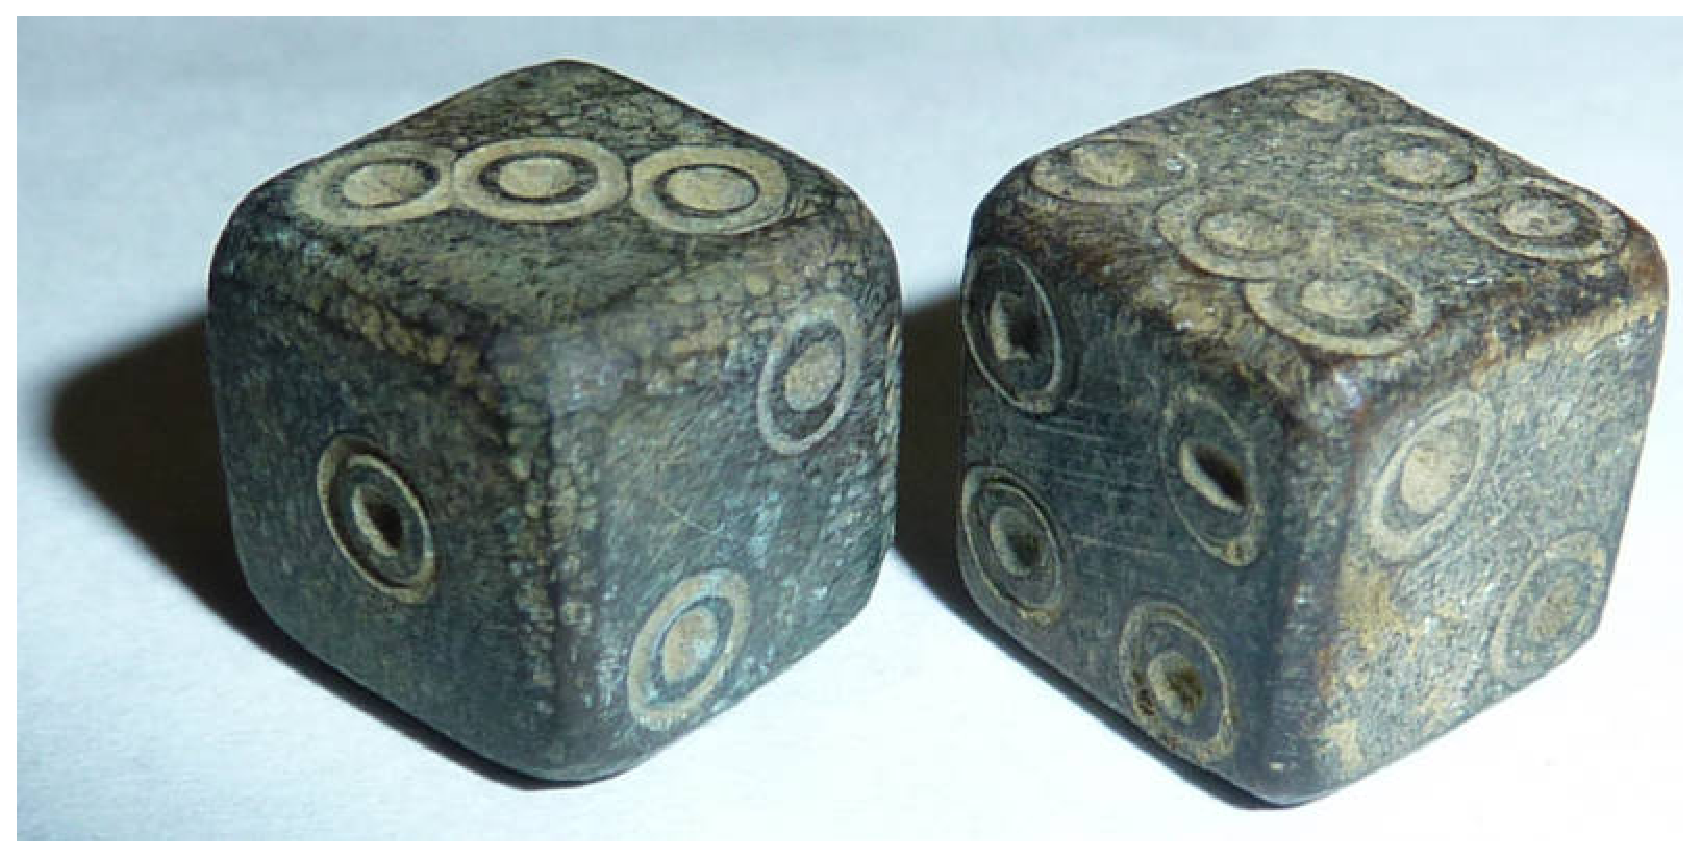
\includegraphics[height=4.2cm]{dice.eps}}
\psframe[linewidth=0.02,linecolor=gray](-6.2,-7)(6.2,2.2)
\psframe[linewidth=0.02,linecolor=gray](-6.15,-6.95)(6.15,2.15)
\rput(0,1.4){\color{myblue}\large Math 207:  Statistics}
\rput(0,0.6){\color{myblue}Chapter 18:  The Normal Approximation for Probability Histograms}
%\psframebox(0,0)(4,4)
\rput(0,-4.5){\scriptsize Dr.~Ralph Wojtowicz}
\rput(0,-5.0){\scriptsize Mathematics Department}
\rput(0,-5.8){
\includegraphics[height=1cm]{su-long.eps}}
%
%\rput(0,-6.5){\scriptsize 17 February 2012}
\end{pspicture}
\end{center}

\end{frame}

%\section[Outline]{}

\addtocounter{page}{-1}
\addtocounter{framenumber}{-1}

{\footnotesize
\frame{\tableofcontents}
}

\section{EV and SE}
\subsection{Law of Averages}

\section{Using the Normal Curve}
\subsection{Using the Normal Curve}
\begin{frame}
\frametitle{Using the Normal Curve}

\footnotesize 

\textbf{Central Limit Theorem}:
When drawing at random with replacement from a box, the probability histogram for the sum
(and the average)
will follow the normal curve, even if the contents of the box do not.  The histogram
must be put into standard units, and the number of draws must be reasonably large.\vspace{-8pt}

\begin{center}
{\setlength{\tabcolsep}{2pt}\begin{tabular}{ccccccc}
$\displaystyle\mbox{EV}_{\mbox{\scriptsize sum}}$ & $=$  & $n\cdot \mbox{AV}_{\mbox{\scriptsize box}}$ & 
   \hspace{.5in}
$\displaystyle\mbox{EV}_{\mbox{\scriptsize av}}$ &  $=$ & $\hphantom{n\cdot }\mbox{AV}_{\mbox{\scriptsize box}}$ \\[5pt]
%
$\displaystyle\mbox{SE}_{\mbox{\scriptsize sum}}$ & $=$ & $\sqrt{n}\cdot \mbox{SD}_{\mbox{\scriptsize box}}$ & 
   \hspace{.5in}
$\displaystyle\mbox{SE}_{\mbox{\scriptsize av}}$  & $=$ & 
  $\frac{\mbox{SD}_{\mbox{\tiny box}}}{\sqrt{n}}$ \\
\end{tabular}}

\begin{tabular}{ccc}
\begin{pspicture}(-3,0)(2,2.5)
\psframe(-3,-1.0)(2.4,2.3)
\psGauss[linecolor=red,mue=-1,sigma=0.4]{-3}{2}
\psGauss[linecolor=blue,mue=-0.5, sigma=0.5]{-2.5}{2}
\psGauss[linecolor=black,mue=0, sigma=0.6]{-2}{2}
\psline{->}(-1,-0.3)(1,-0.3)
\rput(0,-0.6){increasing $n$}
\end{pspicture}
& \hspace{.2in}
\begin{pspicture}(-2,0)(2,2.5)
\psframe(-2.3,-1.0)(2.3,2.3)
\psGauss[linecolor=red,mue=0,sigma=0.4]{-2}{2}
\psGauss[linecolor=blue,mue=0, sigma=0.3]{-2}{2}
\psGauss[linecolor=black,mue=0, sigma=0.2]{-2}{2}
\psline{->}(1.2,0.3)(1.2,1.9)
\rput{90}(1.5,1.12){increasing $n$}
\end{pspicture}

\end{tabular}
\end{center}


\end{frame}

\subsection{Flipping Coins}
\begin{frame}
\frametitle{Five Coins:  Sum of Number of Heads Follows a Normal Curve}

\footnotesize
\texttt{source("BoxSimulations.R")}
\texttt{data = 

\end{frame}

\subsection{Examples II}
\begin{frame}
\frametitle{Examples (II)}

\footnotesize

\begin{itemize}
\item<2-> A die will be tossed 120 times.  What is the chance that the 
    {\color{blue}number} of 4s will be
    between 15 and 25?\\[3pt]

The box model is \scalebox{0.8}{\psframebox{\psframebox{0}\;\psframebox{0}\;\psframebox{0}\;%
   \psframebox{1}\;\psframebox{0}\;\psframebox{0}}}\\[4pt]
    $\mbox{AV}_{\scriptsize\mbox{box}}  = \frac{1}{6}$ and 
    $\mbox{SD}_{\scriptsize\mbox{box}}  = \frac{\sqrt{5}}{6}\approx 0.373$.\\[3pt]
    $\mbox{EV}_{\scriptsize\mbox{sum}}  = 120\cdot \frac{1}{6} = 20$ and 
    $\mbox{SE}_{\scriptsize\mbox{sum}}  = \sqrt{120}\cdot \frac{\sqrt{5}}{6} \approx 4.08$\\[3pt]
    $z_1= \frac{15 - 20}{4.08} = -1.23$ and $z_2 = \frac{25-20}{4.08}=1.23$\\[3pt]
    Chance $= \mbox{pnorm}(1.23)  - \mbox{pnorm}(-1.23) = 0.781=78.1\%$
%
\item<3-> A die will be tossed 12,000 times.  What is the chance that the 
    {\color{darkgreen}percentage} of 4s will be
    between 16\% and 17\%?\\[3pt]
    $\mbox{EV}_{\scriptsize\mbox{av}}= \frac{1}{6} = 0.166667 = 16.7\%$ and 
    $\mbox{SE}_{\scriptsize\mbox{av}}  = \frac{\sqrt{5}}{6}/\sqrt{12000} \approx 0.0034=0.34\%$\\[3pt]
    $z_1= \frac{16 - 16.7}{0.34} = -1.96$ and $z_2 = \frac{17-16.7}{0.34}=0.98$\\[3pt]
    Chance $= \mbox{pnorm}(0.98)  - \mbox{pnorm}(-1.96) = 0.811=81.1\%$
\end{itemize}
\end{frame}

\section{SD Shortcut}
\subsection{SD Shortcut}
\begin{frame}
\frametitle{SD Shortcut}

\footnotesize 

\begin{itemize}
\item If there are only two different numbers on the tickets in a box then we can use
   a shortcut formula to compute the SD of the box.
\end{itemize}
\[\mbox{SD}_{\scriptsize\mbox{box}} = 
\left(\begin{array}{c}\mbox{big}\\\mbox{number}\end{array}\; -\;
   \begin{array}{c}\mbox{small}\\\mbox{number}\end{array}\right)\;
\sqrt{\left(\begin{array}{c}\mbox{fraction of}\\ \mbox{tickets with}\\  \mbox{big number}\end{array}
      \right)\cdot
\left(\begin{array}{c}\mbox{fraction of}\\ \mbox{tickets with}\\  \mbox{small number}\end{array}
  \right)}\]
\begin{itemize}
\item Examples:\vspace{-4pt}
\end{itemize}
\begin{center}
\begin{tabular}{|lcl|}\hline
             & Box & \hfil SD\\\hline
Flipping coins & \scalebox{0.8}{\psframebox{\psframebox{0}\;\psframebox{1}}} & 
        $(1-0)\sqrt{\frac{1}{2}\cdot \frac{1}{2}} = \frac{1}{2} = 0.5$
   \vphantom{\LARGE Y}\\[10pt]
Counting 4s on die rolls & 
   \scalebox{0.8}{\psframebox{\psframebox{0}\;\psframebox{0}\;\psframebox{0}\;\psframebox{1}\;%
\psframebox{0}\;\psframebox{0}\;}} &
   $(1-0)\sqrt{\frac{1}{6}\cdot \frac{5}{6}}= \frac{\sqrt{5}}{6}\approx 0.373$\\[10pt]
Sample from a box & 
     \scalebox{0.8}{\psframebox{\psframebox{-1}\;\psframebox{-1}\;\psframebox{1}\;\psframebox{1}\;%
\psframebox{1}}} & 
  $(1 - (-1))\,\sqrt{\frac{3}{5}\cdot\frac{2}{5}} = \frac{2\,\sqrt{6}}{5}\approx 0.980$\\[10pt]
Sample from a box & 
     \scalebox{0.8}{\psframebox{\psframebox{1}\;\psframebox{3}\;\psframebox{3}\;\psframebox{5}}} & 
  We can't use the shortcut.\\[5pt]\hline
\end{tabular}
\end{center}
\label{lastpage}
\end{frame}
\end{document}

\section{Classifying and Counting}
\subsection{Classifying and Counting}
\begin{frame}
\frametitle{Classifying and Counting}

\end{frame}

\subsection{Examples}
\begin{frame}
\frametitle{Examples}

\end{frame}
\end{document}



\end{frame}
\end{document}
